\documentclass[12pt, twoside]{article}
\documentclass[12pt, twoside]{article}
\usepackage[letterpaper, margin=1in, headsep=0.2in]{geometry}
\setlength{\headheight}{0.6in}
%\usepackage[english]{babel}
\usepackage[utf8]{inputenc}
\usepackage{microtype}
\usepackage{amsmath}
\usepackage{amssymb}
%\usepackage{amsfonts}
\usepackage{siunitx} %units in math. eg 20\milli\meter
\usepackage{yhmath} % for arcs, overparenth command
\usepackage{tikz} %graphics
\usetikzlibrary{quotes, angles}
\usepackage{graphicx} %consider setting \graphicspath{{images/}}
\usepackage{parskip} %no paragraph indent
\usepackage{enumitem}
\usepackage{multicol}
\usepackage{venndiagram}

\usepackage{fancyhdr}
\pagestyle{fancy}
\fancyhf{}
\renewcommand{\headrulewidth}{0pt} % disable the underline of the header
\raggedbottom
\hfuzz=2mm %suppresses overfull box warnings

\usepackage{hyperref}

\fancyhead[LE]{\thepage}
\fancyhead[RO]{\thepage \\ Name: \hspace{4cm} \,\\}
\fancyhead[LO]{BECA / Dr. Huson / Geometry\\*  Unit 8: Regents review\\* 28 May 2025}

\begin{document}

\subsubsection*{8.5 Classwork: Analytic geometry \hfill 8.F.A.3}
\begin{enumerate}

\item A line is plotted in the graph below.
\begin{multicols}{2}
    \begin{enumerate}[itemsep=0.5cm]
      \item Write down the $y$-intercept of the line.
      \item What is the slope of the line?
      \item What is the $x$-intercept of the line?
      \item Write down its equation in slope-intercept form.
      \end{enumerate}
    \begin{flushright}
    \begin{tikzpicture}[scale=0.8]
      \draw [help lines] (-1,-2) grid (6,5);
      \draw [thick, ->] (-1.2,0) -- (6.6,0) node [above right] {$x$};
      \draw [thick, ->] (0,-2.2)--(0,5.4) node [right] {$y$};
      \draw [fill] (0,3) circle [radius=0.07] node[above right] {$(0,3)$};
      \draw [fill] (6,0) circle [radius=0.07] node[below left] {$(6,0)$};
      \draw [<->, thick, domain=-0.5:6.8] plot (\x,-0.5*\x+3);
    \end{tikzpicture}
    \end{flushright}
  \end{multicols} \vspace{2cm}

\item Find the slope of the line through the points $(-1, 4)$ and $(1, 6)$. \vspace{3cm}

\item A line has a slope of $\displaystyle \frac{3}{5}$ and passes through the point $(10, 7)$. 
  \begin{enumerate}[itemsep=1cm]
      \item Write the equation of the line in the form $(y-y_1)=m(x-x_1)$.
      \item Rewrite the equation of the line in the form $y=mx+b$. \vspace{4cm}
  \end{enumerate}

\newpage
\subsubsection*{Systems of equations \hfill HSG.REI.C.6}
\item Graph and label the two equations. Mark their intersection as an ordered pair.
  \begin{multicols}{2}
    $f(x) = -\frac{1}{2}x+4$ \\[1cm]
    $g(x) = \frac{1}{3}x-1$ \\
  \begin{tikzpicture}[scale=.635]
    \draw [help lines] (-2,-2) grid (8,6);
    \draw [thick, ->] (-2.2,0) -- (8.4,0) node [below right] {$x$};
    \draw [thick, ->] (0,-2.2)--(0,6.4) node [left] {$y$};
    %\draw [<->, thick, domain=-1.5:6.8] plot (\x,-0.5*\x+4);
    %\draw [<->, thick, domain=-0.5:6.8] plot (\x,0.3333*\x-1);
  \end{tikzpicture}
\end{multicols}

  
\item Dr. Huson buys six pizza pies for the Pi Day party, some plain, some special with all the toppings. Plain pizzas cost \$10 and ``everything'' pizzas \$15. The total cost was \$75. How many of each pizza did he buy?
\begin{multicols}{2}
Let $x$ be the number of plain pizzas and $y$ be the number of pizzas with everything.
\begin{enumerate}
  \item Write an equation and graph a line to represent a total of six pizzas.
  \item Make a second equation and line representing the \$75 total cost.
  \item Mark the intersection as an ordered pair and state the number of each type of pizza.
\end{enumerate}
  \begin{flushright}
    \begin{tikzpicture}[scale=0.7]
      \draw [help lines] (0,0) grid (10,10);
      \draw [thick, ->] (0,0) -- (10.4,0) node [above ] {$x$};
      \draw [thick, ->] (0,0)--(0,10.4) node [right] {$y$};
      \foreach \x in {1,...,10}
      \draw[shift={(\x,0)}] (0pt,-3pt)--(0pt,3pt) node[below=5pt] {$\x$};
      \foreach \y in {1,...,10}
      \draw[shift={(0,\y)}] (-3pt,0pt)--(3pt,0pt) node[left=5pt] {$\y$};
      %\draw [<->, thick, domain=0:6] plot (\x,-\x+6);
      %\draw [<->, thick, domain=0:7.5] plot (\x,-0.6667*\x+5);
    \end{tikzpicture} \vspace{2cm}
  \end{flushright}
\end{multicols}


\end{enumerate}
\end{document}